% Created 2022-12-21 mer. 11:10
% Intended LaTeX compiler: pdflatex
\documentclass[paper=a4, 12pt, DIV=12]{scrartcl}
\usepackage[utf8]{inputenc}
\usepackage[T1]{fontenc}
\usepackage{graphicx}
\usepackage{longtable}
\usepackage{wrapfig}
\usepackage{rotating}
\usepackage[normalem]{ulem}
\usepackage{amsmath}
\usepackage{amssymb}
\usepackage{capt-of}
\usepackage{hyperref}
\usepackage{minted}
\usepackage{amsfonts}
\usepackage[english]{babel}
\usepackage{bookmark}
\usepackage{xcolor}
\definecolor{pnasblue}{RGB}{0,101,165}
\hypersetup{colorlinks=true, allcolors=pnasblue}
\definecolor{bg}{rgb}{0.95,0.95,0.95}
\author{Ghislain Vieilledent\textsuperscript{\(\ast\), \ddag{}}}
\date{\today}
\title{Using the \texttt{riskmapjnr} Python module to map the deforestation risk following the JNR methodology\\\medskip
\large \textcolor{pnasblue}{First report for FAO focused on small-scale test areas\\ FAO budget code: TF/NFODD/TFGB110021450}}
\hypersetup{
 pdfauthor={Ghislain Vieilledent\textsuperscript{\(\ast\), \ddag{}}},
 pdftitle={Using the \texttt{riskmapjnr} Python module to map the deforestation risk following the JNR methodology},
 pdfkeywords={},
 pdfsubject={},
 pdfcreator={Emacs 28.2 (Org mode 9.5.5)}, 
 pdflang={English}}
\makeatletter
\newcommand{\citeprocitem}[2]{\hyper@linkstart{cite}{citeproc_bib_item_#1}#2\hyper@linkend}
\makeatother

\usepackage[notquote]{hanging}
\begin{document}

\maketitle

\vspace{-1cm}
\begin{center}
  $\ast$ \textbf{Correspondence to:}~ghislain.vieilledent@cirad.fr \\
  $\ddag$ \textbf{CIRAD}, UMR AMAP, F-34398 Montpellier, FRANCE \\
\end{center}
\vspace{0.25cm}

\begin{abstract}
The JNR (Jurisdictional Nested REDD+) provides a standardized approach to estimate and credit greenhouse gas (GHG) emission reductions in the framework of REDD+ (Reducing Emissions from Deforestation and Forest Degradation) programs. The JNR approach relies on a map of the deforestation risk to be able to allocate the deforestation spatially within the jurisdiction when projecting future deforestation under the reference scenario. The JNR Risk Mapping Tool presents a standardized approach to obtain this map of the deforestation risk. The methodology is based on minimal spatial information provided by the past deforestation map at the jurisdictional scale. While the methodology favors simplicity, the approach requires several computationally intensive geoprocessing steps on potentially large raster files. The \texttt{riskmapjnr} Python package we developed provides easy-to-use functions to obtain the risk map following the JNR methodology. Functions use optimized Python code that can efficiently process large raster files without memory issues. Here we provide an example of the use of the \texttt{riskmapjnr} Python package for small-case test areas. \textbf{The package is still under development. The code might include some errors and still need to be thoroughly tested}. A first stable version (v1.0) of the package will be released at the end of the year 2022. As a consequence, \textbf{these preliminary results should be interpreted with caution}.
\end{abstract}

\vspace{0.25cm}
\begin{center}

\includegraphics[width=0.86\textwidth]{images/partners_logos.png}\enlargethispage{2\baselineskip}
\end{center}
\newpage
\tableofcontents
\newpage
\listoffigures
\newpage

\section{Introduction}
\label{sec:org68c1eaa}

\subsection{Context}
\label{sec:org5e6a61b}

In the forest sector, programs to mitigate GHG emissions across entire national or subnational jurisdictions (called \href{https://redd.unfccc.int/}{REDD+} programs, i.e. programs aiming at Reducing Emissions from Deforestation and Forest Degradation) can be accounted for and credited using a jurisdictional-scale framework called \href{https://verra.org/project/jurisdictional-and-nested-redd-framework/}{JNR} (Jurisdictional and Nested REDD+). JNR integrates government-led and project-level REDD+ activities and establishes a clear pathway for subnational- and project-level activities to be incorporated within broader REDD+ programs. The JNR framework ensures all projects and other reducing emissions from deforestation and degradation activities in a given jurisdiction are developed using consistent baselines and crediting approaches. They mitigate the risk of ``leakage'', i.e. the displacement of emission-causing activities to areas outside the project boundary, by monitoring emissions across an entire jurisdictional area. JNR is part of the \href{https://verra.org/project/vcs-program/}{VCS} (Verified Carbon Standard) program which allows certified projects to turn their greenhouse gas (GHG) emission reductions and removals into tradable carbon credits. Since its launch in 2006, the VCS program has grown into the world's largest voluntary GHG program.

The \href{https://verra.org/wp-content/uploads/2021/04/DRAFT\_JNR\_Risk\_Mapping\_Tool\_15APR2021.pdf}{JNR Risk Mapping Tool} is a ``benchmark'' methodology that provides a standardized approach for developing deforestation and forest degradation risk maps for users of the \href{https://verra.org/wp-content/uploads/2021/04/JNR\_Allocation\_Tool\_Guidance\_v4.0.pdf}{JNR Allocation Tool} in the context of JNR requirements. The methodology allows deriving a map of the deforestation (or degradation) risk based on a minimal spatial information provided by the past deforestation (or degradation) map at the jurisdictional scale. The \href{https://verra.org/wp-content/uploads/2021/04/DRAFT\_JNR\_Risk\_Mapping\_Tool\_15APR2021.pdf}{JNR Risk Mapping Tool} allows the creation of categorical and spatially static maps whose categories represent different levels of risk of deforestation or forest degradation in the validity period of the Forest Reference Emissions Level (FREL) and throughout the jurisdictional geographical boundaries. In the \href{https://verra.org/wp-content/uploads/2021/04/JNR\_Allocation\_Tool\_Guidance\_v4.0.pdf}{JNR Allocation Tool}, the level of risk determines how the jurisdictional FREL is spatially distributed to nested lower-level jurisdictional programs and projects.

\subsection{Objectives}
\label{sec:orgb4ced9b}

While the \href{https://verra.org/wp-content/uploads/2021/04/DRAFT\_JNR\_Risk\_Mapping\_Tool\_15APR2021.pdf}{JNR Risk Mapping Tool} methodology favors simplicity, obtaining the risk map is not straightforward. The approach requires several geoprocessing steps on raster data that can be large, i.e. covering large spatial extent (eg. national scale) at high spatial resolution (eg. 30 m). The \texttt{riskmapjnr} Python package we developed includes functions to perform these geoprocessing steps and derive a risk map on any jurisdiction and at any spatial resolution following the \href{https://verra.org/wp-content/uploads/2021/04/DRAFT\_JNR\_Risk\_Mapping\_Tool\_15APR2021.pdf}{JNR Risk Mapping Tool} methodology. The \texttt{riskmapjnr} package includes functions to:

\begin{enumerate}
\item Estimate the distance to forest edge beyond which the deforestation risk is negligible: \texttt{dist\_edge\_threshold()}.
\item Compute local deforestation rates using a moving window whose size can vary: \texttt{local\_defor\_rate()}.
\item Transform local deforestation rates into categories of deforestation risks using several slicing algorithms: \texttt{set\_defor\_cat\_zero()} and \texttt{defor\_cat()}
\item Validate maps of deforestation risk and select the map with the higher accuracy: \texttt{defrate\_per\_cat()} and \texttt{validation()}.
\end{enumerate}

The \texttt{riskmapjnr} package uses several known Python scientific packages such as \texttt{NumPy}, \texttt{SciPy}, and \texttt{Pandas} for fast matrix and vector operations and \texttt{gdal} for processing georeferenced raster data. Raster data are divided into blocks of data for in-memory processing. Such an approach allow processing large raster files with large geographical extents (e.g. country scale) and high spatial resolutions (eg. 30 m). Here we present an example of the use of the \texttt{riskmapjnr} Python package for small-case test areas following all the steps of the JNR methodology.

\subsection{Warnings}
\label{sec:orge82f17e}

The \texttt{riskmapjnr}  package is still under development. The code might include some errors and still need to be thoroughly tested. A first stable version (v1.0) of the package will be released at the end of the year 2022. As a consequence, the preliminary results presented here should be interpreted with caution. Moreover, the JNR methodology is currently discussed and will be subject to changes in the coming months. Future versions of the \texttt{riskmapjnr} package should integrate these changes.

\section{Initial setup and data}
\label{sec:org31e851b}

\subsection{Installation}
\label{sec:orgaea432c}

You need several dependencies to run the \texttt{riskmapjnr} Python package. The best way to install the package is to create a Python virtual environment, either through \texttt{conda} (recommended) or \texttt{virtualenv}.

\begin{enumerate}
\item Using \texttt{conda} (recommended)
\label{sec:org9a4f3b1}

You first need to have \texttt{miniconda3} installed (see \href{https://docs.conda.io/en/latest/miniconda.html}{miniconda instructions}). Then, create a conda environment (see \href{https://docs.conda.io/projects/conda/en/latest/user-guide/tasks/manage-environments.html}{conda environment instructions}) and install the \texttt{riskmapjnr} package with the following commands:

\begin{minted}[breaklines=true,bgcolor=bg]{shell}
conda create --name conda-rmj -c conda-forge python=3 gdal numpy matplotlib pandas pip scipy --yes
conda activate conda-rmj
pip install riskmapjnr # For PyPI version
# pip install https://github.com/ghislainv/riskmapjnr/archive/master.zip # For GitHub dev version
# conda install -c conda-forge jupyter geopandas descartes folium --yes  # Optional additional packages
\end{minted}

To deactivate and delete the conda environment:

\begin{minted}[breaklines=true,bgcolor=bg]{shell}
conda deactivate
conda env remove --name conda-rmj
\end{minted}

\item Using \texttt{virtualenv}
\label{sec:orgc9bc797}

You first need to have the \texttt{virtualenv} package installed (see \href{https://packaging.python.org/guides/installing-using-pip-and-virtual-environments/}{virtualenv instructions}). Then, create a virtual environment and install the \texttt{riskmapjnr} package with the following commands:

\begin{minted}[breaklines=true,bgcolor=bg]{shell}
cd ~
mkdir venvs # Directory for virtual environments
cd venvs
virtualenv --python=/usr/bin/python3 venv-rmj
source ~/venvs/venv-rmj/bin/activate
# Install numpy first
pip install numpy
# Install gdal (the correct version) 
pip install --global-option=build_ext --global-option="-I/usr/include/gdal" gdal==$(gdal-config --version)
pip install riskmapjnr # For PyPI version, this will install all other dependencies
# pip install https://github.com/ghislainv/riskmapjnr/archive/master.zip # For GitHub dev version
# pip install jupyter geopandas descartes folium # Optional additional packages
\end{minted}

To deactivate and delete the virtual environment:

\begin{minted}[breaklines=true,bgcolor=bg]{shell}
deactivate
rm -R ~/venvs/venv-rmj # Just remove the repository
\end{minted}

\item Installation testing
\label{sec:org9365d69}

You can test that the package has been correctly installed using the command \texttt{riskmapjnr} in a terminal:

\begin{minted}[breaklines=true,bgcolor=bg]{shell}
riskmapjnr
\end{minted}

This should return a short description of the \texttt{riskmapjnr} package and the version number:

\begin{minted}[breaklines=true,bgcolor=bg]{shell}
# riskmapjnr: Map of deforestation risk following JNR methodology.
# https://ecology.ghislainv.fr/riskmapjnr/
# riskmapjnr version x.x.
\end{minted}

You can also test the package executing the commands in the \href{https://ecology.ghislainv.fr/riskmapjnr/notebooks/get\_started.html}{Get started} tutorial of the \href{https://ecology.ghislainv.fr/riskmapjnr}{\texttt{riskmapjnr} website}.
\end{enumerate}

\subsection{Importing Python modules}
\label{sec:orgc22b72a}

We import the Python modules needed for running the analysis.

\begin{minted}[breaklines=true,bgcolor=bg]{python}
# Imports
import os
import multiprocessing as mp
import pkg_resources

import numpy as np
import matplotlib.pyplot as plt
import pandas as pd
from tabulate import tabulate

import riskmapjnr as rmj
\end{minted}

Increase the cache for GDAL to increase computational speed.

\begin{minted}[breaklines=true,bgcolor=bg]{python}
# GDAL
os.environ["GDAL_CACHEMAX"] = "1024"
\end{minted}

Set the \texttt{PROJ\_LIB} environmental variable.

\begin{minted}[breaklines=true,bgcolor=bg]{python}
os.environ["PROJ_LIB"] = os.path.join(
    "/home/ghislain/.pyenv/versions/miniconda3-latest/",
    "envs/conda-rmj/share/proj")
\end{minted}

Create a directory to save the results.

\begin{minted}[breaklines=true,bgcolor=bg]{python}
out_dir = "outputs"
rmj.make_dir(out_dir)
\end{minted}

\subsection{Forest cover change data}
\label{sec:org0c454ec}

We use the Guadeloupe archipelago as a case study. Recent forest cover change data for Guadeloupe is included in the \texttt{riskmapjnr} package. The raster file (\texttt{fcc123\_GLP.tif}) includes the following values: \textbf{1} for deforestation in the period 2000--2010, \textbf{2} for deforestation in the period 2010--2020, and \textbf{3} for the remaining forest in 2020. NoData value is set to \textbf{0}. The first period (2000--2010) will be used for calibration and the second period (2010--2020) will be used for validation. This is the only data we need to derive a map of deforestation risk following the JNR methodology.

\begin{minted}[breaklines=true,bgcolor=bg]{python}
fcc_file = pkg_resources.resource_filename(
    "riskmapjnr",
    "data/fcc123_GLP.tif")
print(fcc_file)
border_file = pkg_resources.resource_filename(
    "riskmapjnr",
    "data/ctry_border_GLP.gpkg")
print(border_file)
\end{minted}

We plot the forest cover change map with the \texttt{plot.fcc123()} function.

\begin{minted}[breaklines=true,bgcolor=bg]{python}
ofile = os.path.join(out_dir, "fcc123.png")
fig_fcc123 = rmj.plot.fcc123(
    input_fcc_raster=fcc_file,
    maxpixels=1e8,
    output_file=ofile,
    borders=border_file,
    linewidth=0.2,
    figsize=(5, 4), dpi=800)
ofile
\end{minted}

\begin{figure}[H]
\centering
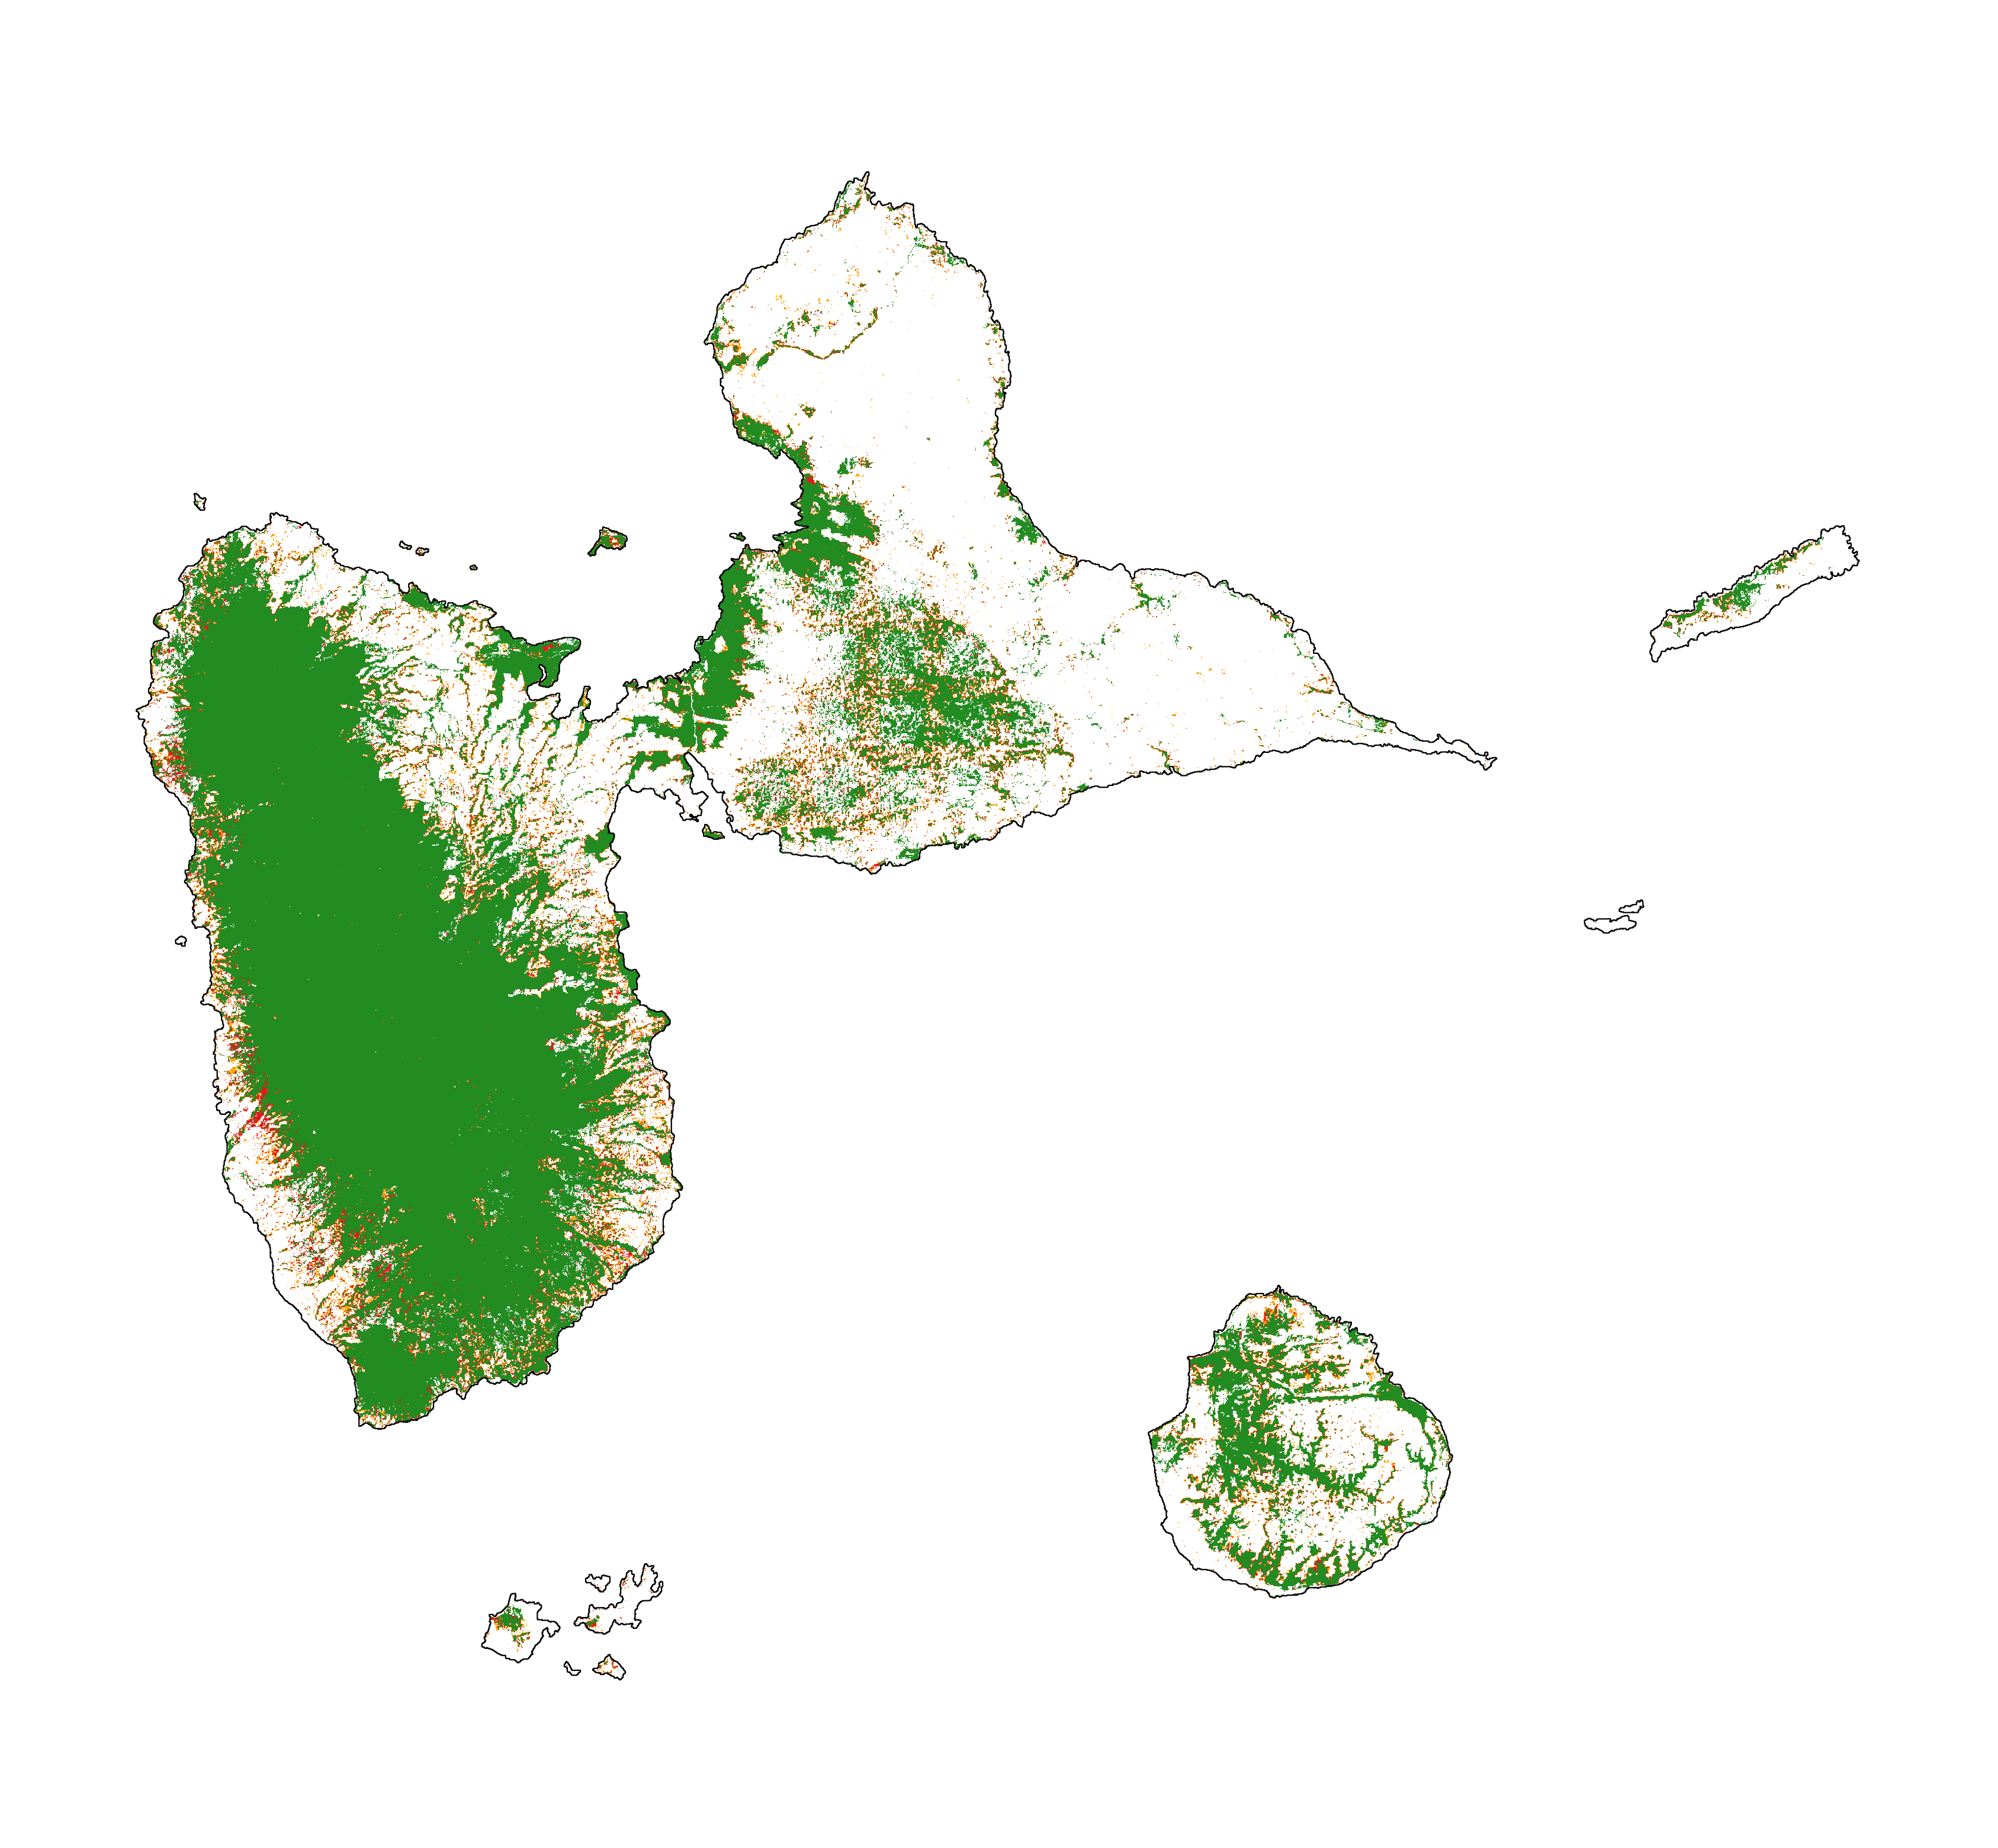
\includegraphics[width=0.8\linewidth]{outputs/fcc123.png}
\caption{\label{fig:org985ab5f}\textbf{Forest cover change map.} Deforestation on the first period (2000--2010) is in orange, deforestation on the second period (2000--2020) is in red and remaining forest (in 2020) is in green.}
\end{figure}

\section{Steps to derive a categorical map of deforestation risk}
\label{sec:orgeef0c1b}

\subsection{Deforestation risk with distance to forest edge}
\label{sec:org08bff6f}

The first step is to compute the distance to the forest edge after which the risk of deforestation becomes negligible. Indeed, it is known from previous studies on tropical deforestation that the deforestation risk decreases rapidly with the distance to the forest edge and that most of the deforestation occurs close to the forest edge (\citeprocitem{4}{Vieilledent et al. 2013}, \citeprocitem{5}{2022}, \citeprocitem{1}{Dezécache et al. 2017}, \citeprocitem{2}{Grinand et al. 2020}). The JNR methodology suggests identifying the distance to the forest edge \(d\), so that at least 99\% of the deforestation occurs within a distance \(\leq d\). Forest areas located at a distance from the forest edge \(> d\) can be considered as having no risk of being deforested. As a consequence, forest pixels with a distance from the forest edge \(> d\) are assigned category 0 (zero) for the deforestation risk. The threshold distance can be computed with the function \texttt{dist\_edge\_threshold()}.

\begin{minted}[breaklines=true,bgcolor=bg]{python}
ofile = os.path.join(out_dir, "perc_dist_steps.png")
dist_edge_thres_steps = rmj.dist_edge_threshold(
    fcc_file=fcc_file,
    defor_values=1,
    dist_file=os.path.join(out_dir, "dist_edge_steps.tif"),
    dist_bins=np.arange(0, 1080, step=30),
    tab_file_dist=os.path.join(out_dir, "tab_dist_steps.csv"),
    fig_file_dist=ofile,
    blk_rows=128, verbose=False)
ofile
\end{minted}

\begin{figure}[H]
\centering
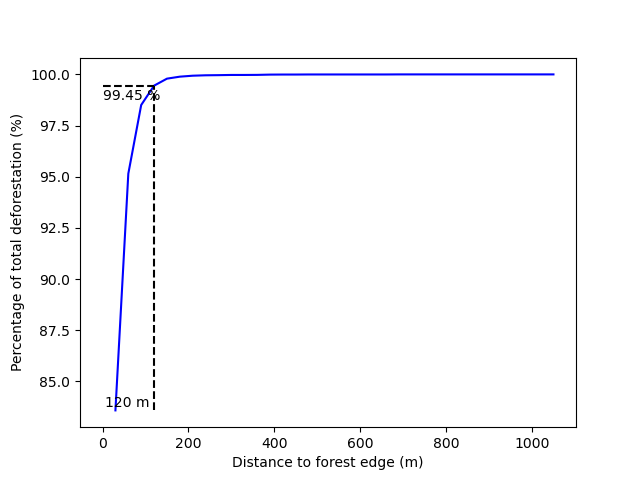
\includegraphics[width=0.8\linewidth]{outputs/perc_dist_steps.png}
\caption{\label{fig:org69512a9}\textbf{Identifying areas for which the risk of deforestation is negligible.} Figure shows that more than 99\% of the deforestation occurs within a distance from the forest edge \(\leq 120\) m. Forest areas located at a distance \(> 120\) m from the forest edge can be considered as having no risk of being deforested.}
\end{figure}

The function returns a dictionary including the distance threshold:

\begin{minted}[breaklines=true,bgcolor=bg]{python}
dist_thresh = dist_edge_thres_steps["dist_thresh"]
print(f"The distance threshold is {dist_thresh} m")
\end{minted}

\begin{verbatim}
The distance threshold is 120 m
\end{verbatim}


A table indicating the cumulative percentage of deforestation as a function of the distance is also produced:

\begin{center}
\begin{tabular}{rrrrr}
Distance & Npixels & Area & Cumulation & Percentage\\
\hline
30 & 24937 & 2244.33 & 2244.33 & 83.583\\
60 & 3451 & 310.59 & 2554.92 & 95.15\\
90 & 1001 & 90.09 & 2645.01 & 98.5051\\
120 & 282 & 25.38 & 2670.39 & 99.4503\\
150 & 102 & 9.18 & 2679.57 & 99.7922\\
180 & 29 & 2.61 & 2682.18 & 99.8894\\
210 & 14 & 1.26 & 2683.44 & 99.9363\\
240 & 6 & 0.54 & 2683.98 & 99.9564\\
270 & 2 & 0.18 & 2684.16 & 99.9631\\
300 & 3 & 0.27 & 2684.43 & 99.9732\\
\end{tabular}
\end{center}

\subsection{Local deforestation rate}
\label{sec:orgc2799e2}

The second step computes a local risk of deforestation at the pixel level using a moving window made of several pixels. The deforestation risk is estimated from the deforestation rate inside the moving window. The deforestation rate \(\theta\) (in \%/yr) is computed from the formula \(\theta=1-(\alpha_2/\alpha_1)^{1/\tau}\), with \(\alpha\) the forest areas (in ha) at time \(t_1\) and \(t_2\), and \(\tau\), the time interval (in yr) between time \(t_1\) and \(t_2\). Using the deforestation rate formula, the moving window and the past forest cover change map, we can derive a raster map describing the local risk of deforestation at the same resolution as the input map. To save space on disk, deforestation rates are converted to integer values between 0 and 10000 (ten thousand) and the raster type is set to UInt16. This ensures a precision of 10\textsuperscript{-4} for the deforestation rate which is sufficient to determine the 30 categories of deforestation risk, as imposed by the JNR methodology.

\begin{minted}[breaklines=true,bgcolor=bg]{python}
# Set window size
s = 21
# Compute local deforestation rate
rmj.local_defor_rate(
    fcc_file=fcc_file,
    defor_values=1,
    ldefrate_file=os.path.join(out_dir, f"ldefrate_steps.tif"),
    win_size=s,
    time_interval=10,
    blk_rows=100,
    verbose=False)
\end{minted}

\subsection{Pixels with zero risk of deforestation}
\label{sec:orgd415b45}

This third step sets a value of 10001 to pixels with zero deforestation risk. As explained previously, a risk of deforestation of zero is assumed when distance to forest edge is greater than the distance below which more than 99\% of the deforestation occurs.

\begin{minted}[breaklines=true,bgcolor=bg]{python}
rmj.set_defor_cat_zero(
    ldefrate_file=os.path.join(out_dir, f"ldefrate_steps.tif"),
    dist_file=os.path.join(out_dir, "dist_edge_steps.tif"),
    dist_thresh=dist_thresh,
    ldefrate_with_zero_file=os.path.join(
        out_dir, f"ldefrate_with_zero_steps.tif"),
    blk_rows=128,
    verbose=False)
\end{minted}

\subsection{Categories of deforestation risk}
\label{sec:orgeb91e51}

The fourth step implies converting the continuous values of the raster map of deforestation risk to categorical values. The JNR methodology suggests to use 31 classes of risk from ``0'' to ``30'' including the ``0'' class for the forest pixels with no risk of being deforested (located at a distance to the forest edge \(> d\), see first step). Following the JNR methodology, at least three slicing algorithms must be compared to derive the categorical map of deforestation risk, such as ``equal area'', ``equal interval'', and ``natural breaks''. With the ``equal area'' algorithm, each class from ``1'' to ``30'' must cover approximately the same area. With the ``equal interval'' algorithm, classes from ``1'' to ``30'' correspond to bins of deforestation risk of the same range. In this case, some risk classes will be in majority in the landscape compared to other classes of lower frequency. With the ``natural breaks'' algorithm, the continuous deforestation risk is normalized before running an ``equal interval'' algorithm. To perform this step, we use the function \texttt{defor\_cat()} which returns the corresponding bins of deforestation probability.

\begin{minted}[breaklines=true,bgcolor=bg]{python}
bins = rmj.defor_cat(
    ldefrate_with_zero_file=os.path.join(
        out_dir, f"ldefrate_with_zero_steps.tif"),
    riskmap_file=os.path.join(out_dir, "riskmap_steps.tif"),
    ncat=30,
    method="Equal Area",
    blk_rows=128,
    verbose=False)
\end{minted}

The risk map can be plotted using the \texttt{plot.riskmap()} function.

\begin{minted}[breaklines=true,bgcolor=bg]{python}
ofile = os.path.join(out_dir, "riskmap_steps.png")
riskmap_fig = rmj.plot.riskmap(
    input_risk_map=os.path.join(out_dir, "riskmap_steps.tif"),
    maxpixels=1e8,
    output_file=ofile,
    borders=border_file,
    legend=True,
    figsize=(5, 4), dpi=800,
    linewidth=0.2,)
ofile
\end{minted}

\begin{figure}[H]
\centering
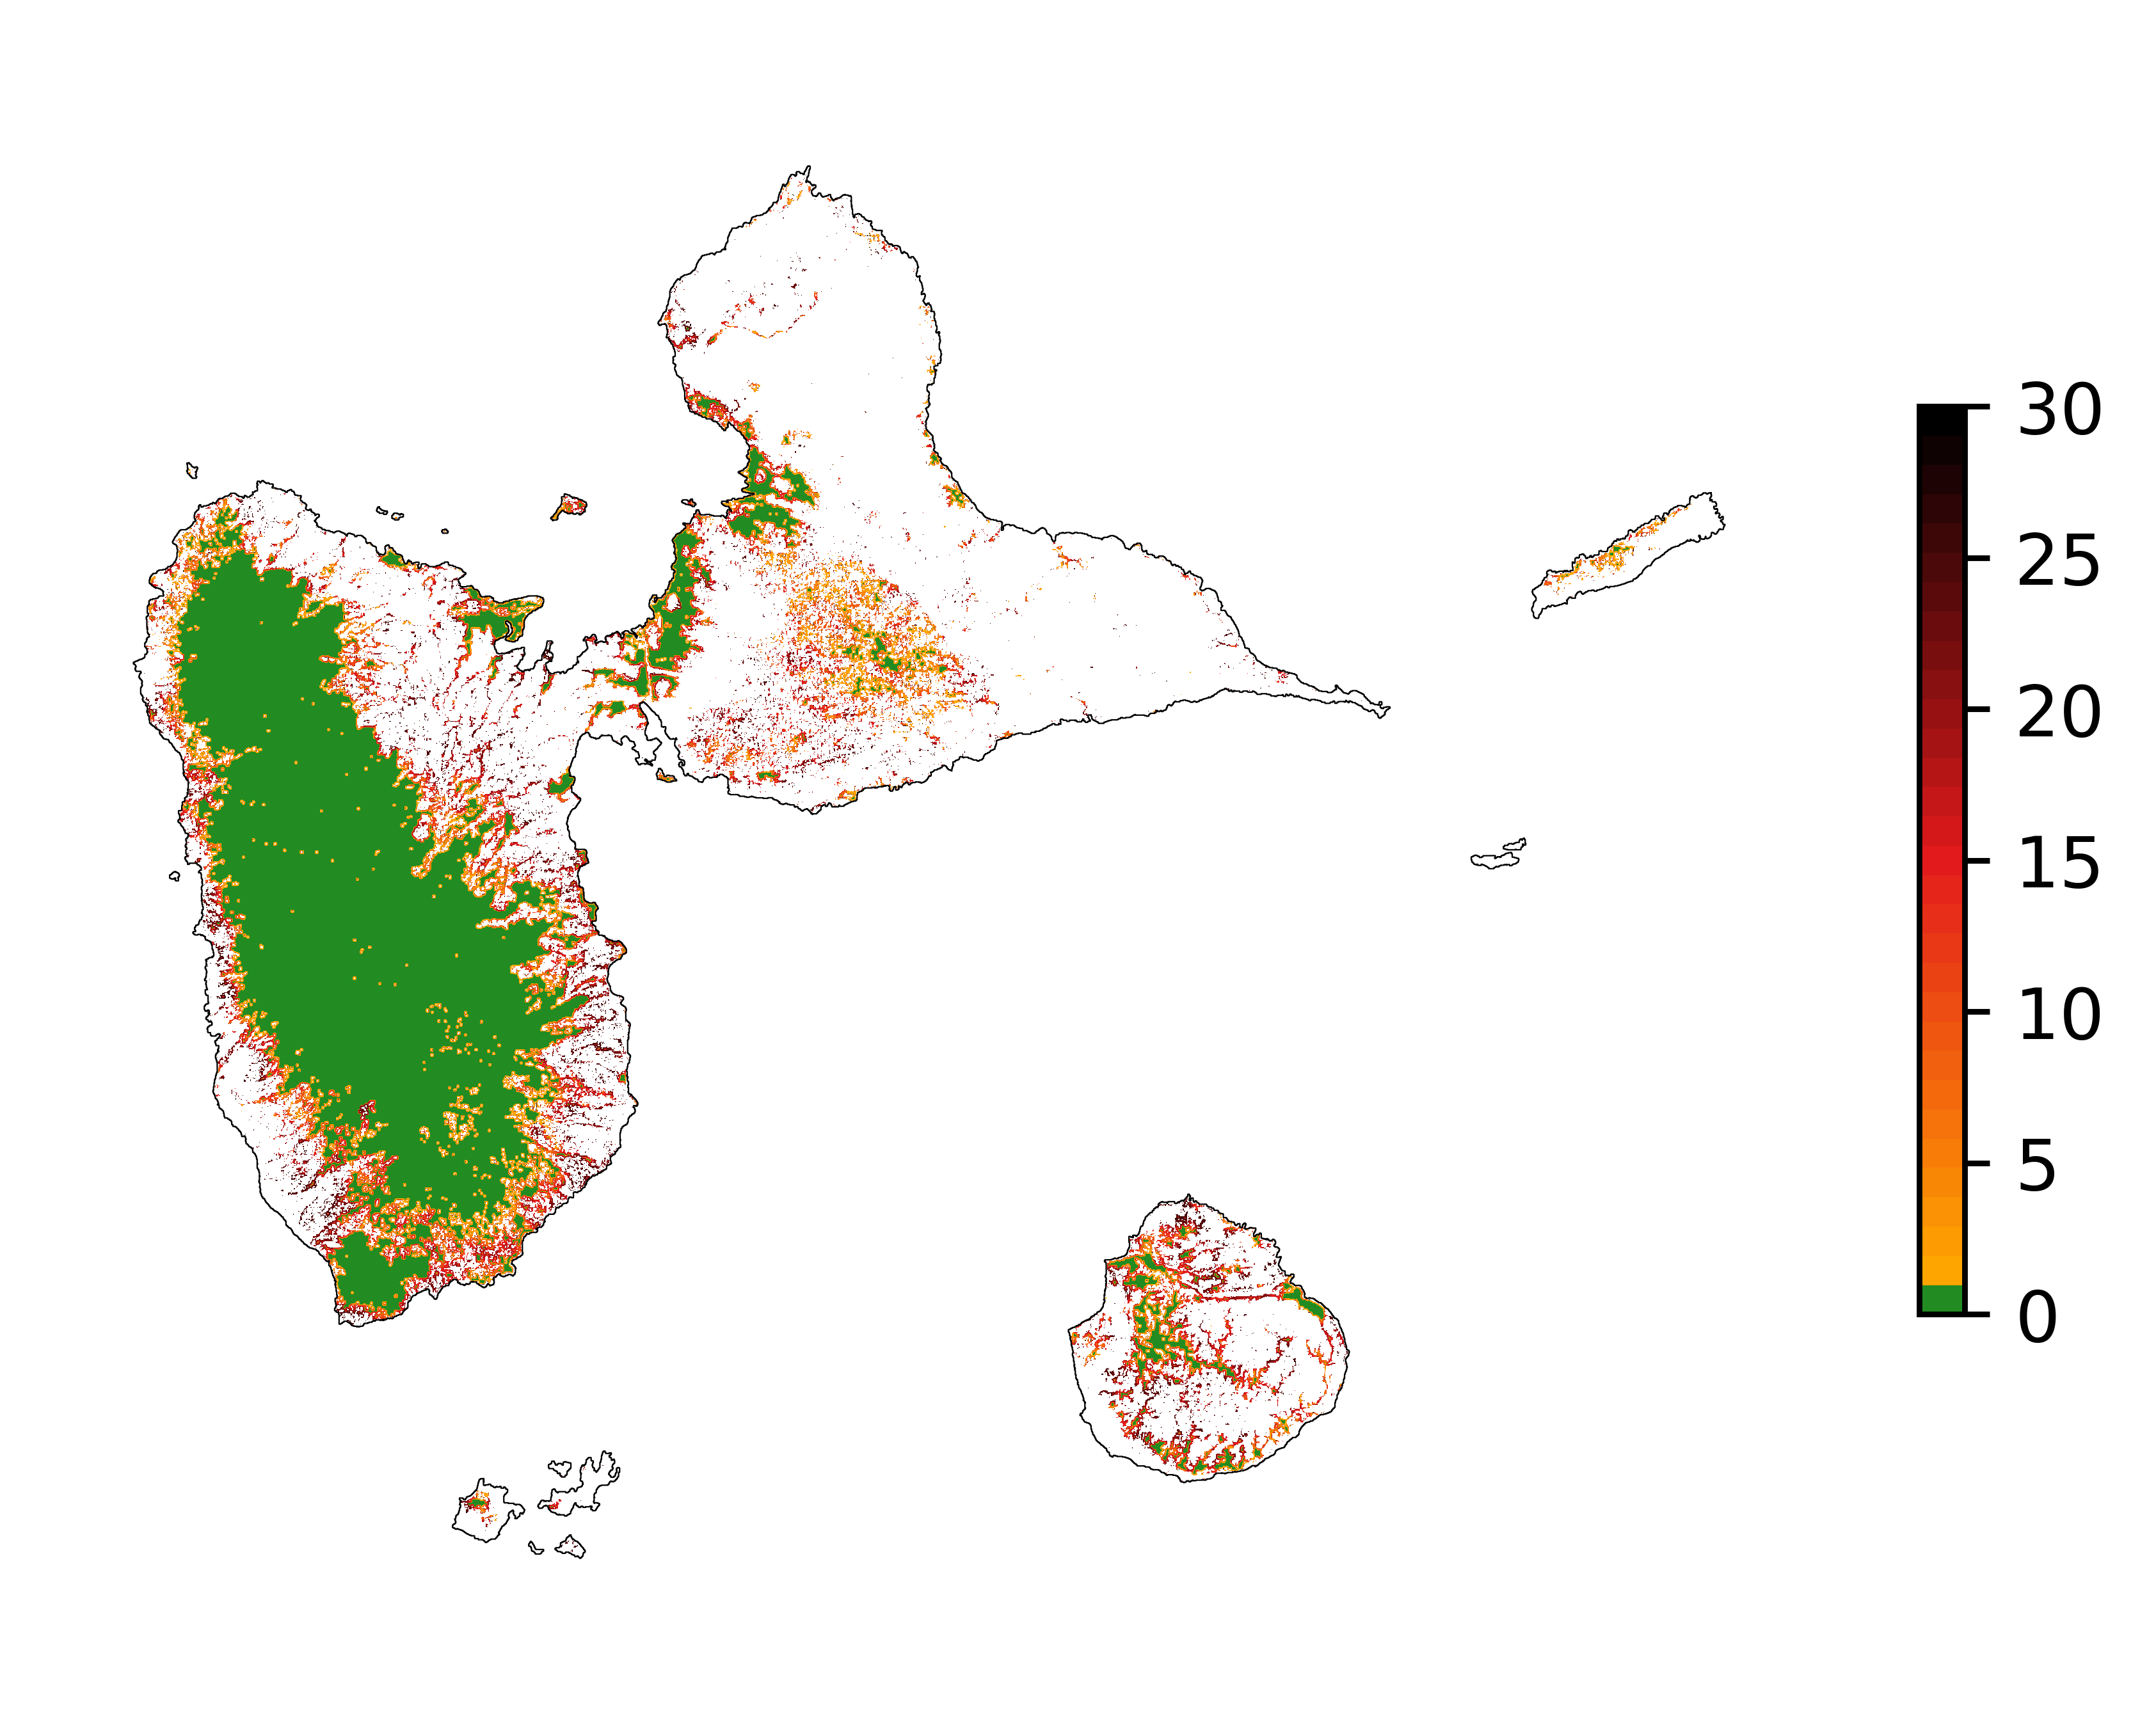
\includegraphics[width=0.8\linewidth]{outputs/riskmap_steps.png}
\caption{\label{fig:org0d68add}\textbf{Map of the deforestation risk following the JNR methodology}. Forest pixels are categorized in up to 30 classes of deforestation risk. Forest pixels which belong to the class 0 (in green) are located farther than a distance of 120 m from the forest edge and have a negligible risk of being deforested.}
\end{figure}

\subsection{Deforestation rates per category of risk}
\label{sec:orgdd28805}

Before the validation step, we need to compute the historical deforestation rates (in \%/yr) for each category of spatial deforestation risk. The historical deforestation rates are computed for the calibration period (here 2000--2010). Deforestation rates provide estimates of the percentage of forest (which is then converted to an area of forest) that should be deforested inside each forest pixel which belongs to a given category of deforestation risk.

\begin{minted}[breaklines=true,bgcolor=bg]{python}
rmj.defrate_per_cat(
    fcc_file=fcc_file,
    defor_values=1,
    riskmap_file=os.path.join(out_dir, "riskmap_steps.tif"),
    time_interval=10,
    tab_file_defrate=os.path.join(out_dir, "defrate_per_cat_steps.csv"),
    blk_rows=128,
    verbose=False)
\end{minted}

A table indicating the deforestation rate per category of deforestation is produced:

\begin{center}
\begin{tabular}{rrrr}
cat & nfor & ndefor & rate\\
\hline
1 & 70257 & 0 & 0\\
2 & 17189 & 47 & 0.000273768\\
3 & 4258 & 15 & 0.000352838\\
4 & 15311 & 92 & 0.000602506\\
5 & 17683 & 110 & 0.000623815\\
6 & 11130 & 105 & 0.000947425\\
7 & 14920 & 177 & 0.00119271\\
8 & 12727 & 164 & 0.00129613\\
9 & 14891 & 265 & 0.00179401\\
10 & 13132 & 299 & 0.00230055\\
11 & 14465 & 426 & 0.00298481\\
12 & 13178 & 465 & 0.00358592\\
13 & 13776 & 528 & 0.00390051\\
14 & 14171 & 670 & 0.00483168\\
15 & 13476 & 665 & 0.00504783\\
16 & 12955 & 740 & 0.00586445\\
17 & 13664 & 1032 & 0.00782238\\
18 & 13135 & 1101 & 0.00871624\\
19 & 13244 & 1383 & 0.0109683\\
20 & 13504 & 1520 & 0.0118703\\
21 & 13482 & 1969 & 0.0156639\\
22 & 13273 & 2491 & 0.0205709\\
23 & 13219 & 3053 & 0.0259188\\
24 & 13364 & 4382 & 0.0389551\\
25 & 13171 & 7915 & 0.0877714\\
\end{tabular}
\end{center}

From this table, we see that the deforestation rate increases with the deforestation risk category which is expected. We also see that the ``Equal Area'' slicing algorithm provides categories with similar forest cover at the beginning of the period (see similar values in the ``nfor'' column).

\subsection{Derive a risk map at the beginning of the validation period}
\label{sec:orga655438}

To derive the risk map at the beginning of the validation period, we consider (i) the forest cover at this date, (ii) the map of local deforestation rates, (ii) the threshold distance, and (iii) the bins used to categorize the deforestation rates. All these data are obtained from previous steps and based on the deforestation for the historical period. The approach is the following: first, we consider the forest cover at the beginning of the validation period. Second, we assign category zero to pixels at a distance from the forest edge which is greater than the distance threshold. Third, we categorize the deforestation rates using the previous bins identified for the historical period. In addition to the risk map, two additional raster files are produced: the raster file of the distance to forest edge at the beginning of the validation period, and the raster file of local deforestation rates including the zero deforestation risk.

\begin{enumerate}
\item Distance to forest edge at the beginning of the validation period
\label{sec:orgca6a48d}

\begin{minted}[breaklines=true,bgcolor=bg]{python}
rmj.dist_values(input_file=fcc_file,
                dist_file=os.path.join(out_dir, "dist_edge_v_steps.tif"),
                values="0,1",
                verbose=False)
\end{minted}

\item Raster of local deforestation rate at the beginning of the validation period
\label{sec:org07944a6}

\begin{minted}[breaklines=true,bgcolor=bg]{python}
rmj.get_ldefz_v(
    ldefrate_file=os.path.join(out_dir, "ldefrate_steps.tif"),
    dist_v_file=os.path.join(out_dir, "dist_edge_v_steps.tif"),
    dist_thresh=120,
    ldefrate_with_zero_v_file=os.path.join(out_dir, "ldefrate_with_zero_v_steps.tif"),
    blk_rows=128,
    verbose=False)
\end{minted}

\item Risk map at the beginning of the validation period
\label{sec:org998fb7f}

\begin{minted}[breaklines=true,bgcolor=bg]{python}
rmj.get_riskmap_v(
    ldefrate_with_zero_v_file=os.path.join(out_dir, "ldefrate_with_zero_v_steps.tif"),
    bins=bins,  
    riskmap_v_file=os.path.join(out_dir, "riskmap_v_steps.tif"),
    blk_rows=128,
    verbose=False)
\end{minted}
\end{enumerate}


\section{Map validation}
\label{sec:org4aec4b3}

\subsection{Without correcting for quantity disagreement}
\label{sec:org43f2fff}

The fifth step focuses on comparing the map of deforestation risk with a deforestation map corresponding to the validation period. The validation period follows the calibration period and provides independent observations of deforestation. To do so, we consider a square grid of at least 1000 spatial cells containing at least one forest pixel at the beginning of the validation period. Following JNR specifications, the cell size should be \(\leq\) 10 km. Note that with the map of deforestation risk, each forest pixel at the beginning of the validation period falls into a category of deforestation risk. For each cell of the grid, we compute the predicted area of deforestation (in ha) given the map of deforestation risk and the historical deforestation rates for each category of deforestation risk computed on the calibration period (see previous step). We can then compare the predicted deforestation with the observed deforestation in that spatial cell for the validation period. Because all cells don't have the same forest cover at the beginning of the validation period, a weight \(w_j\) is computed for each grid cell \(j\) such that \(w_j=\beta_j / B\), with \(\beta_j\) the forest cover (in ha) in the cell \(j\) at the beginning of the validation period and \(B\) the total forest cover in the jurisdiction (in ha) at the same date. We then calculate the weighted root mean squared error (wRMSE) from the observed and predicted deforestation for each cell and the cell weights.

\begin{minted}[breaklines=true,bgcolor=bg]{python}
ofile = os.path.join(out_dir, "pred_obs_steps.png")
rmj.validation(
    fcc_file=fcc_file,
    time_interval=10,
    riskmap_file=os.path.join(out_dir, "riskmap_v_steps.tif"),
    tab_file_defrate=os.path.join(out_dir, "defrate_per_cat_steps.csv"),
    csize=40,
    tab_file_pred=os.path.join(out_dir, "pred_obs_steps.csv"),
    fig_file_pred=ofile,
    figsize=(6.4, 4.8),
    dpi=100, verbose=False)
ofile
\end{minted}

\begin{figure}[H]
\centering
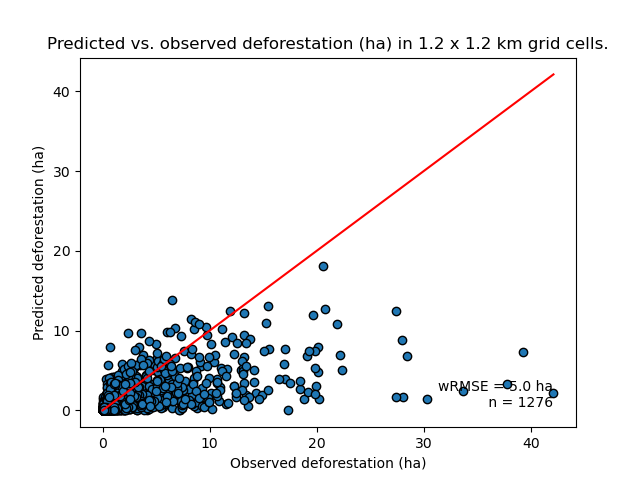
\includegraphics[width=0.8\linewidth]{outputs/pred_obs_steps.png}
\caption{\label{fig:org090da09}\textbf{Relationship between observed and predicted deforestation in 1 x 1 km grid cells}. The red line is the identity line. Values of the weighted root mean squared error (wRMSE, in ha) and of the number of observations (\(n\), the number of spatial cells) are reported on the graph.}
\end{figure}

\subsection{Correcting for quantity disagreement}
\label{sec:orgd9a32c1}

We set the argument \texttt{no\_quantity\_error} to \texttt{True} to correct the total deforestation for the predictions and avoid a ``quantity'' error (\emph{sensu} Pontius) due to the difference in total deforestation between the calibration and validation periods. This is currently being discussed for improving the JNR methodology.

\begin{minted}[breaklines=true,bgcolor=bg]{python}
ofile = os.path.join(out_dir, "pred_obs_corrected_steps.png")
rmj.validation(
    fcc_file=fcc_file,
    time_interval=10,
    riskmap_file=os.path.join(out_dir, "riskmap_v_steps.tif"),
    tab_file_defrate=os.path.join(out_dir, "defrate_per_cat_steps.csv"),
    csize=40,
    no_quantity_error=True,
    tab_file_pred=os.path.join(out_dir, "pred_obs_corrected_step.csv"),
    fig_file_pred=ofile,
    figsize=(6.4, 4.8),
    dpi=100, verbose=False)
ofile
\end{minted}

\begin{figure}[H]
\centering
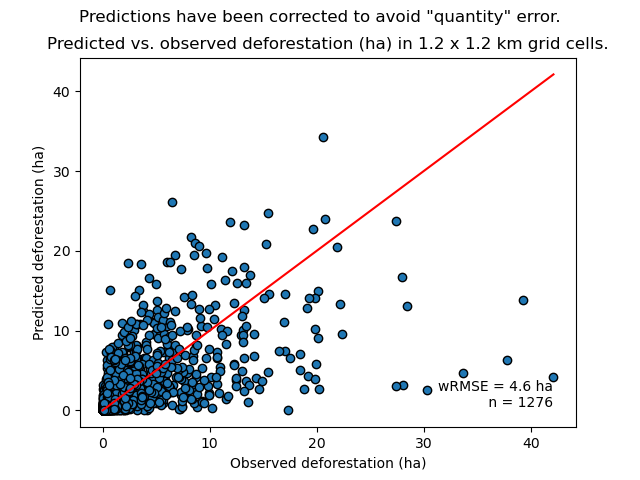
\includegraphics[width=0.8\linewidth]{outputs/pred_obs_corrected_steps.png}
\caption{\label{fig:org0c9a8a1}\textbf{Relationship between observed and predicted deforestation in 1 x 1 km grid cells \emph{after correction for quantity disagreement}}. The red line is the identity line. Values of the weighted root mean squared error (wRMSE, in ha) and of the number of observations (\(n\), the number of spatial cells) are reported on the graph.}
\end{figure}

\section{Final risk map}
\label{sec:org189726c}

\subsection{Obtaining several categorical maps with the \texttt{makemap} function}
\label{sec:org9ac5046}

The user must repeat the procedure detailed above and obtain risk maps for varying window size and slicing algorithms. Following the JNR methodology, at least 25 different sizes for the moving window must be tested together with two slicing algorithms (``Equal Interval'' and ``Equal Area''), thus leading to a minimum of 50 different maps of deforestation risk. The map with the smallest wRMSE value is considered the best risk map. Once the best risk map is identified, with the corresponding window size and slicing algorithm, a final risk map is derived considering both the calibration and validation period. The \texttt{makemap()} function can be used to run all the procedure with varying window size and slicing algorithm. This function calls a sequence of functions from the \texttt{riskmapjnr} package which perform all the steps detailed in the JNR methodology. The function can use parallel computing on several CPUs to reduce computation time. In this case, each map is obtained and validated on one CPU. 

\begin{minted}[breaklines=true,bgcolor=bg]{python}
ncpu = mp.cpu_count() - 2
print(f"Number of CPUs to use: {ncpu}.") 
\end{minted}

\begin{verbatim}
Number of CPUs to use: 6.
\end{verbatim}


\begin{minted}[breaklines=true,bgcolor=bg]{python}
results_makemap = rmj.makemap(
    fcc_file=fcc_file,
    time_interval=[10, 10],
    output_dir=out_dir,
    clean=False,
    dist_bins=np.arange(0, 1080, step=30),
    win_sizes=np.arange(5, 295, 16),
    ncat=30,
    parallel=True,
    ncpu=ncpu,
    methods=["Equal Interval", "Equal Area"],
    csize=40,
    no_quantity_error=True,
    figsize=(6.4, 4.8),
    dpi=100,
    blk_rows=300,  # Set blk_rows > win_size to avoid error
    verbose=True)
\end{minted}

\begin{verbatim}
Model calibration and validation
.. Model 0: window size = 5, slicing method = ei.
.. Model 2: window size = 21, slicing method = ei.
.. Model 4: window size = 37, slicing method = ei.
.. Model 6: window size = 53, slicing method = ei.
.. Model 8: window size = 69, slicing method = ei.
.. Model 10: window size = 85, slicing method = ei.
.. Model 1: window size = 5, slicing method = ea.
.. Model 3: window size = 21, slicing method = ea.
.. Model 5: window size = 37, slicing method = ea.
.. Model 9: window size = 69, slicing method = ea.
.. Model 11: window size = 85, slicing method = ea.
.. Model 7: window size = 53, slicing method = ea.
.. Model 12: window size = 101, slicing method = ei.
.. Model 14: window size = 117, slicing method = ei.
.. Model 16: window size = 133, slicing method = ei.
.. Model 18: window size = 149, slicing method = ei.
.. Model 20: window size = 165, slicing method = ei.
.. Model 22: window size = 181, slicing method = ei.
.. Model 13: window size = 101, slicing method = ea.
.. Model 15: window size = 117, slicing method = ea.
.. Model 19: window size = 149, slicing method = ea.
.. Model 17: window size = 133, slicing method = ea.
.. Model 23: window size = 181, slicing method = ea.
.. Model 21: window size = 165, slicing method = ea.
.. Model 24: window size = 197, slicing method = ei.
.. Model 26: window size = 213, slicing method = ei.
.. Model 30: window size = 245, slicing method = ei.
.. Model 28: window size = 229, slicing method = ei.
.. Model 32: window size = 261, slicing method = ei.
.. Model 34: window size = 277, slicing method = ei.
.. Model 25: window size = 197, slicing method = ea.
.. Model 27: window size = 213, slicing method = ea.
.. Model 31: window size = 245, slicing method = ea.
.. Model 29: window size = 229, slicing method = ea.
.. Model 35: window size = 277, slicing method = ea.
.. Model 33: window size = 261, slicing method = ea.
.. Model 36: window size = 293, slicing method = ei.
.. Model 37: window size = 293, slicing method = ea.
Deriving risk map for full historical period
\end{verbatim}

\subsection{Updated deforestation risk with distance to forest edge}
\label{sec:org8863b95}

We obtain the threshold for the distance to forest edge beyond which the deforestation risk is negligible. Because the time period has changed (now we consider the entire period from 2000 to 2020), the distance threshold has increased from 120 to 180 m.

\begin{minted}[breaklines=true,bgcolor=bg]{python}
dist_thresh = results_makemap["dist_thresh"]
print(f"The distance theshold is {dist_thresh} m.")
\end{minted}

\begin{verbatim}
The distance theshold is 180 m.
\end{verbatim}


We have access to the table indicating the cumulative percentage of deforestation as a function of the distance to forest edge.

We also have access to a plot showing how the cumulative percentage of deforestation increases with the distance to forest edge.

\begin{minted}[breaklines=true,bgcolor=bg]{python}
os.path.join(out_dir, "fullhist/perc_dist.png")
\end{minted}

\begin{figure}[H]
\centering
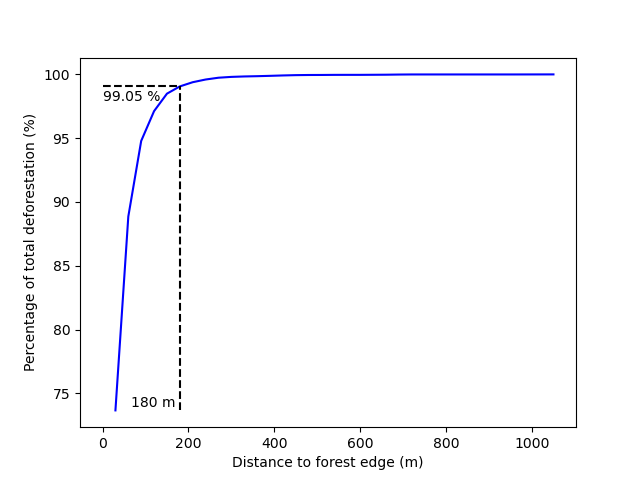
\includegraphics[width=0.8\linewidth]{outputs/fullhist/perc_dist.png}
\caption{\label{fig:org3fa102b}\textbf{Identifying areas for which the risk of deforestation is negligible.} Figure shows that more than 99\% of the deforestation occurs within a distance from the forest edge \(\leq\) 180 m. Forest areas located at a distance > 180 m from the forest edge can be considered as having no risk of being deforested.}
\end{figure}

\subsection{Model comparison}
\label{sec:org529946e}

We can plot the change in wRMSE value with both the window size and slicing algorithm. It seems that the ``Equal Interval'' (ei) algorithm provides lower wRMSE values. The lowest wRMSE value is obtained for the lowest window size. 

\begin{minted}[breaklines=true,bgcolor=bg]{python}
os.path.join(out_dir, f"modcomp/mod_comp.png")
\end{minted}

\begin{figure}[H]
\centering
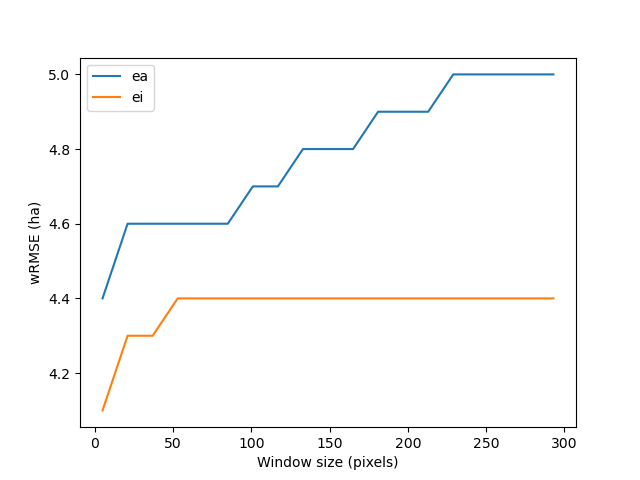
\includegraphics[width=0.8\linewidth]{outputs/modcomp/mod_comp.png}
\caption{\label{fig:org55e06d5}\textbf{Change in wRMSE values as a function of both window size and slicing algorithm}. ``ei'' is the ``Equal Interval'' algorithm and ``ea'' is the ``Equal Area'' algorithm.}
\end{figure}

We identify the moving window size and the slicing algorithm of the best model.

\begin{minted}[breaklines=true,bgcolor=bg]{python}
ws_hat = results_makemap["ws_hat"]
m_hat = results_makemap["m_hat"]
print(f"The best moving window size is {ws_hat} pixels.")
print(f"The best slicing algorithm is '{m_hat}'.")
\end{minted}

\begin{verbatim}
The best moving window size is 5 pixels.
The best slicing algorithm is 'ei'.
\end{verbatim}

\subsection{Model performance}
\label{sec:org75327bd}

We can look at the relationship between observed and predicted deforestation in 1 x 1 km grid cells for the best model.

\begin{minted}[breaklines=true,bgcolor=bg]{python}
os.path.join(out_dir, f"modcomp/pred_obs_ws{ws_hat}_{m_hat}.png")
\end{minted}

\begin{figure}[H]
\centering
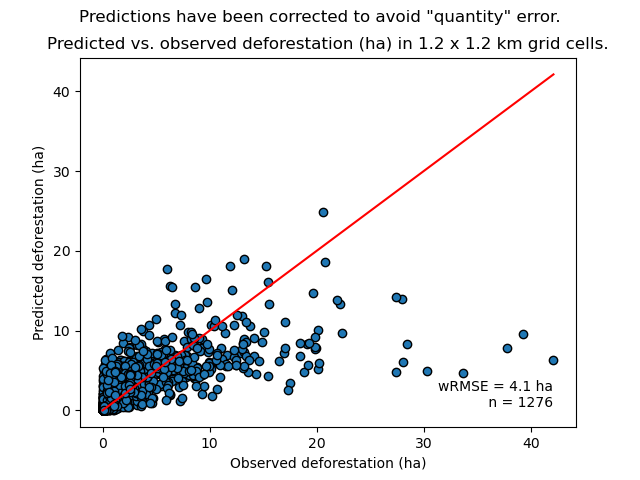
\includegraphics[width=0.8\linewidth]{outputs/modcomp/pred_obs_ws5_ei.png}
\caption{\label{fig:org3781ddb}\textbf{Relationship between observed and predicted deforestation in 1 x 1 km grid cells for the best model}. The red line is the identity line. Values of the weighted root mean squared error (wRMSE, in ha) and of the number of observations (\(n\), the number of spatial cells) are reported on the graph.}
\end{figure}

\subsection{Risk map of deforestation}
\label{sec:orga49e1c2}

We plot the final risk map using the \texttt{plot.riskmap()} function.

\begin{minted}[breaklines=true,bgcolor=bg]{python}
ifile = os.path.join(out_dir, f"endval/riskmap_ws{ws_hat}_{m_hat}_ev.tif")
ofile = os.path.join(out_dir, f"endval/riskmap_ws{ws_hat}_{m_hat}_ev.png")
riskmap_fig = rmj.plot.riskmap(
    input_risk_map=ifile,
    maxpixels=1e8,
    output_file=ofile,
    borders=border_file,
    legend=True,
    figsize=(5, 4), dpi=800, linewidth=0.2,)
ofile
\end{minted}

\begin{figure}[H]
\centering
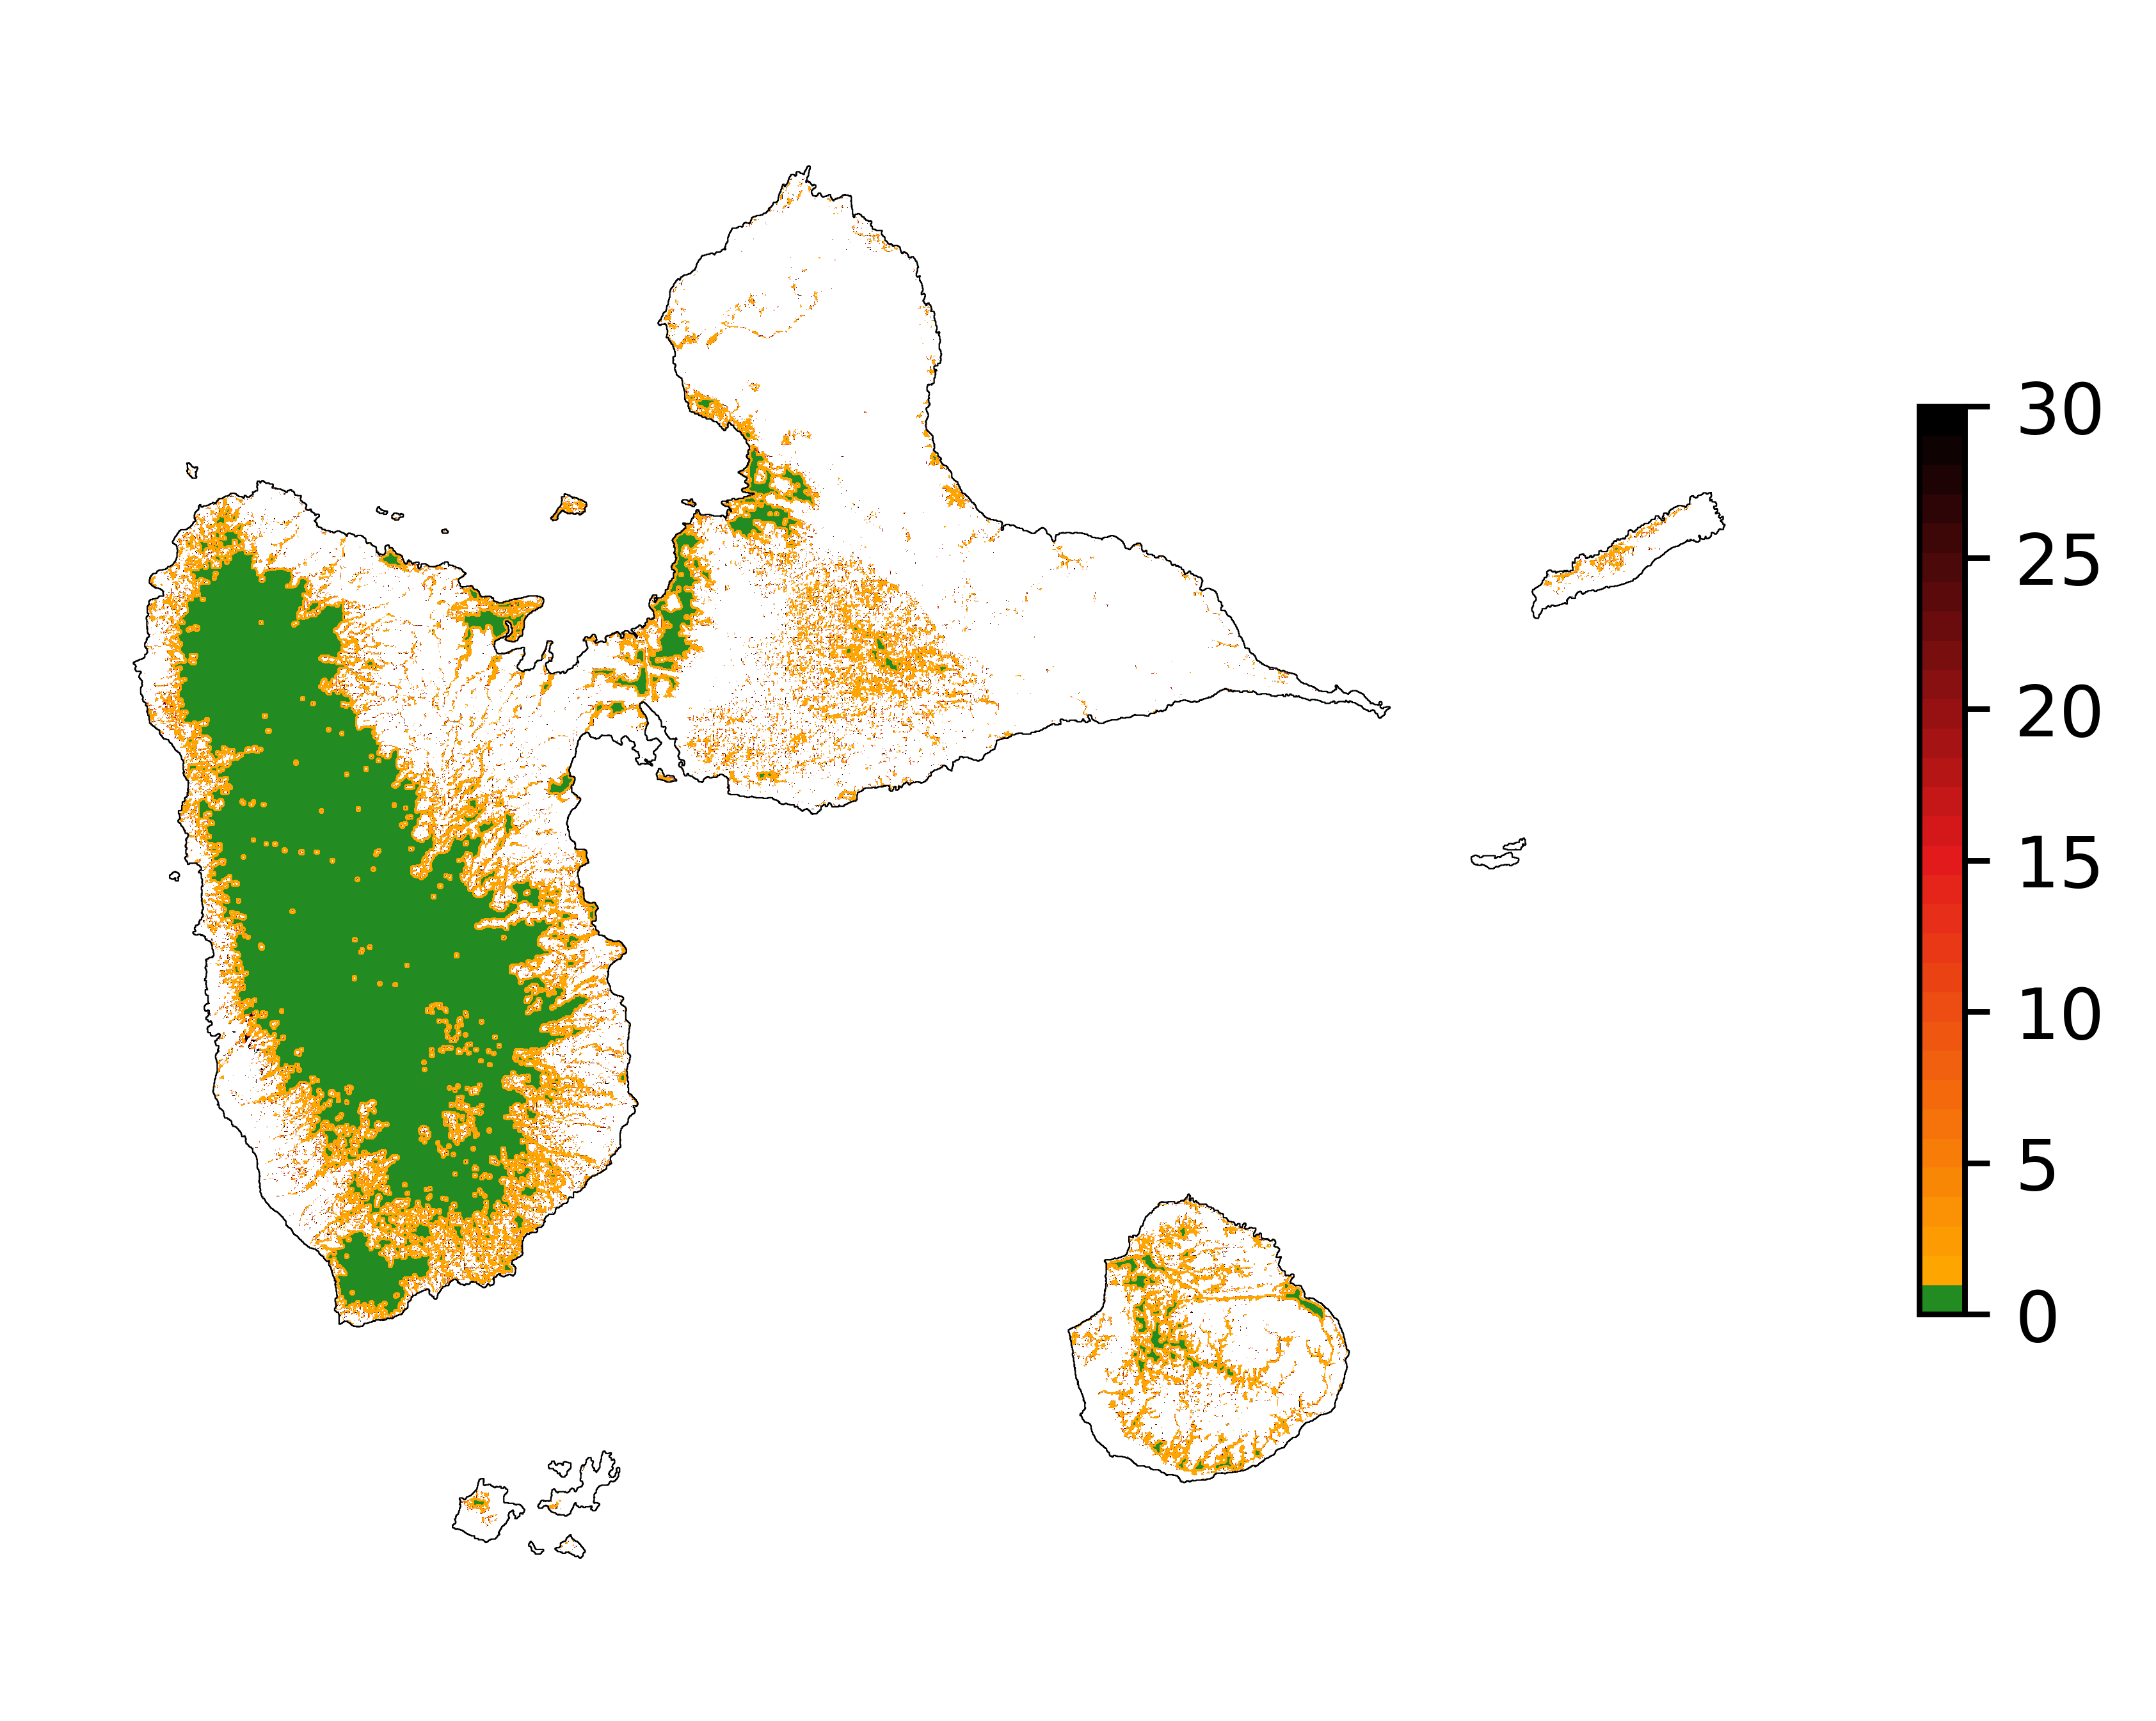
\includegraphics[width=0.8\linewidth]{outputs/endval/riskmap_ws5_ei_ev.png}
\caption{\label{fig:org39b9a3d}\textbf{Map of the deforestation risk following the JNR methodology}. Forest pixels are categorized in up to 30 classes of deforestation risk. Forest pixels which belong to the class 0 (in green) are located farther than a distance of 180 m from the forest edge and have a negligible risk of being deforested.}
\end{figure}

\section{Conclusion}
\label{sec:org043e4ec}

We have presented the use of the \texttt{riskmapjnr} Python package to obtain a map of the deforestation risk following the JNR methodology. As said previously, the JNR methodology is currently being discussed and will likely be subject to changes. The first results we have obtained applying the JNR methodology to a small-scale study area allow us to make some recommendations regarding how the JNR methodology could be improved to obtain an accurate map of the deforestation risk. First, the distance threshold above which deforestation become negligible is changing between the calibration period and the whole period (combining the calibration and validation periods) for the final risk map. This is unavoidable as the deforestation generally progresses towards the forest core and the whole period to derive the final map is longer than the calibration period. Here we used the second distance threshold value of 180 m identified using forest cover change data for the whole period 2000--2020. The JNR methodology should be more precise regarding the distance threshold which should be used. Second, it seems that the ``Equal Area'' slicing algorithm always provides higher wRMSE values than compared with the ``Equal Interval'' algorithm (Fig. \ref{fig:org55e06d5}). As, a consequence, it might be useless to compute maps using this slicing algorithm. This result must be confirmed with other case studies. Third, there is a large underestimation of the total amount of deforestation for the validation period (Fig. \ref{fig:org3781ddb}). To be able to properly compare deforestation risk maps (each map providing a different way of allocating deforestation spatially \emph{sensu} Pontius and Millones (\citeprocitem{3}{2011})) there should be no quantity error between deforestation predictions and observations (\emph{sensu} Pontius and Millones (\citeprocitem{3}{2011})). We suggest not mixing quantity and allocation of deforestation for predictions while the methodology suggests to estimate historical deforestation rates for each category of risk from the calibration period. On the contrary, for the prediction, we suggest to fix the intensity of the deforestation to the one observed on the validation period and use the risk map to identify pixels which should be deforested first. 

\section{References}
\label{sec:orgb00c599}

\begin{hangparas}{1.5em}{1}
\hypertarget{citeproc_bib_item_1}{Dezécache, C., J.-M. Salles, G. Vieilledent, and B. Hérault. 2017. \href{https://doi.org/10.1111/gcb.13611}{Moving forward socio-economically focused models of deforestation}. Global change biology 23:3484–3500.}

\hypertarget{citeproc_bib_item_2}{Grinand, C., G. Vieilledent, T. Razafimbelo, J.-R. Rakotoarijaona, M. Nourtier, and M. Bernoux. 2020. \href{https://doi.org/10.1002/ldr.3526}{Landscape-scale spatial modelling of deforestation, land degradation, and regeneration using machine learning tools}. Land degradation \& development 31:1699–1712.}

\hypertarget{citeproc_bib_item_3}{Pontius, R. G. J., and M. Millones. 2011. \href{https://doi.org/10.1080/01431161.2011.552923}{Death to Kappa: birth of quantity disagreement and allocation disagreement for accuracy assessment}. International journal of remote sensing 32:4407–4429.}

\hypertarget{citeproc_bib_item_4}{Vieilledent, G., C. Grinand, and R. Vaudry. 2013. \href{https://doi.org/10.1002/ece3.550}{Forecasting deforestation and carbon emissions in tropical developing countries facing demographic expansion: a case study in Madagascar}. Ecology and evolution 3:1702–1716.}

\hypertarget{citeproc_bib_item_5}{Vieilledent, G., C. Vancutsem, C. Bourgoin, P. Ploton, P. Verley, and F. Achard. 2022. \href{https://doi.org/10.1101/2022.03.22.485306}{Spatial scenario of tropical deforestation and carbon emissions for the 21st century}. Biorxiv.}
\end{hangparas}
\end{document}